\chapter{Manejo de Aguas Residuales}
% Promedio de DQO: 250ml/L, lo que representa el 0.25\%,
En importante enfatizar sobre los procesos de tratamiento con factibilidad económico, técnico y cultural; también sobre el peligro a la salud por el uso de aguas contaminadas, proporcionar normatividad en cuanto al vertido y reúso de las aguas residuales

\begin{definition}[Aguas residuales]
    Las aguas de composición variada provenientes de las descargas de usos municipales, industriales, comerciales, de servicios, agrícolas, pecuarios, etc.
\end{definition}
La disponibilidad es más elocuente, sis e relaciona con la región y su población, por ejemplo:
\begin{table}[h!]
    \centering
    \begin{tabular}{@{}cc@{}}
    \toprule
    País    & $m^3$   \\ \midrule
    Canadá  & 109,000 \\
    Rusia & 15,000  \\
    USA     & 10,000  \\
    México  & 5,200   \\
    Arabia  & 160     \\
    Egipto  & 30      \\
    Israel  & 330     \\ \bottomrule
    \end{tabular}
    \caption{Metros cúbicos anuales por habitante}
    \label{mar1}
\end{table}
El 50\% del volumen escurrido se genera en tan solo el 20\% de la superficie del país localizada en el sureste mientras que el 4\% del escurrimiento se genera en la parte norte del país en una superficie del 30\% en México
recordando que el agua tiene enlaces de hidrógeno, propiedad de solvente del agua, pH, etc. Se analizarán las características físicas del agua como el olor, color, sabor, turbiedad, temperatura y contenido de sólidos; las características químicas tienen sustancias inorgánicas, pH, alcalinidad, contenido de metales pesados, compuestos tóxicos, sustancias orgánicas, proteínas, grasas, carbohidratos, detergentes, gases, oxígeno, $co_2$, metano, $H_2S$; las características biológicas tiene como actores las bacterias, hongos, algas, protozoarios y virus.

Hablar del agua, sus beneficios y problemática implica  analizar, global y localmente, aquellos factores que afectan su cantidad y calidad, entre otros: la contaminación,  la alteración del clima, las cantidades crecientes de basura cada vez mas toxica.

El 50\% del volumen escurrido se genera en tan solo el 20\% de la superficie del país localizada en el sureste, mientras que el 4\% del escurrimiento se genera en la parte norte del país en una superficie del orden del 30\% del territorio nacional.

\subsection{Naturaleza y composición de las aguas residuales}
El origen de los contaminantes son urbano, industrial, agrícola, pecuario y natural; los cuales están contaminadas por sólidos en suspensión, químicos limpiadores con presencia de altos contenidos de sustancias contaminantes, pesticidas y plaguicidas, fertilizantes y abonos

\begin{definition}[Aguas negras]
    Contienen orina y heces fecales (Inodoros y urinales)
\end{definition}

\begin{definition}[Aguas grises]
    Principalmente contienen detergentes y grasas, provienen de lavaplatos, lavadoras, lavabos y lavaderos
\end{definition}
\begin{definition}[Aguas verdes]
    Son resultado de los procesos que se llevan a cabo en el sector secundario de la economía, es decir el referido a las actividades industriales.
\end{definition}
\subsubsection{Características de los contaminantes de las aguas residuales}
\begin{itemize}
    \item Sus características físicas son que tienen olor, color, sabor, turbiedad, temperatura y contenidos de sólidos.
    \item Las características químicas son sustancias inorgánicas, pH, alcalinidad, contenido de metales pesados, compuestos tóxicos, compuestos orgánicos, proteínas, grasas, carbohidratos, detergentes, gases, oxígeno, $CO_2$, metano, $H_2S$, etc.
    \item Características biológicas: Bacterias, hongos, virus, algas y protozoarios.
\end{itemize}

\subsubsection{Muestreo de aguas residuales}
\begin{itemize}
    \item Sitios de muestreo
    \item Técnicas de muestreo
    \item Frecuencia de muestreo (análisis estadístico)
\end{itemize}
Los principales indicadores e índices de contaminación, están dadas por:
\begin{itemize}
    \item Demanda Bioquímica de Oxígeno (DBO)
    \item Demanda Química de Oxígeno (DQO)
    \item Demanda Teórica de Oxígeno (DTO)
\end{itemize}
\begin{table}[h!]
    \centering
    \begin{tabular}{@{}cc@{}}
    \toprule
    Estado                          & $DBO_5\quad mg/L$ \\ \midrule
    Agua pura                       & 0-20              \\
    Agua levemente contaminada      & 20-100            \\
    Agua medianamente contaminada   & 100-500           \\
    Agua muy contaminada            & 500-3,000         \\
    Agua extremadamente contaminada & 3,000-5,000       \\ \bottomrule
    \end{tabular}
    \caption{Demanda Bioquímica de Oxígeno (DBO), cantidad de oxígeno que se debe proporcionar a las bacterias para descomponer el agua y poder tratarla}
    \label{tabar1}
\end{table}

\begin{figure}[h!]
\centering
  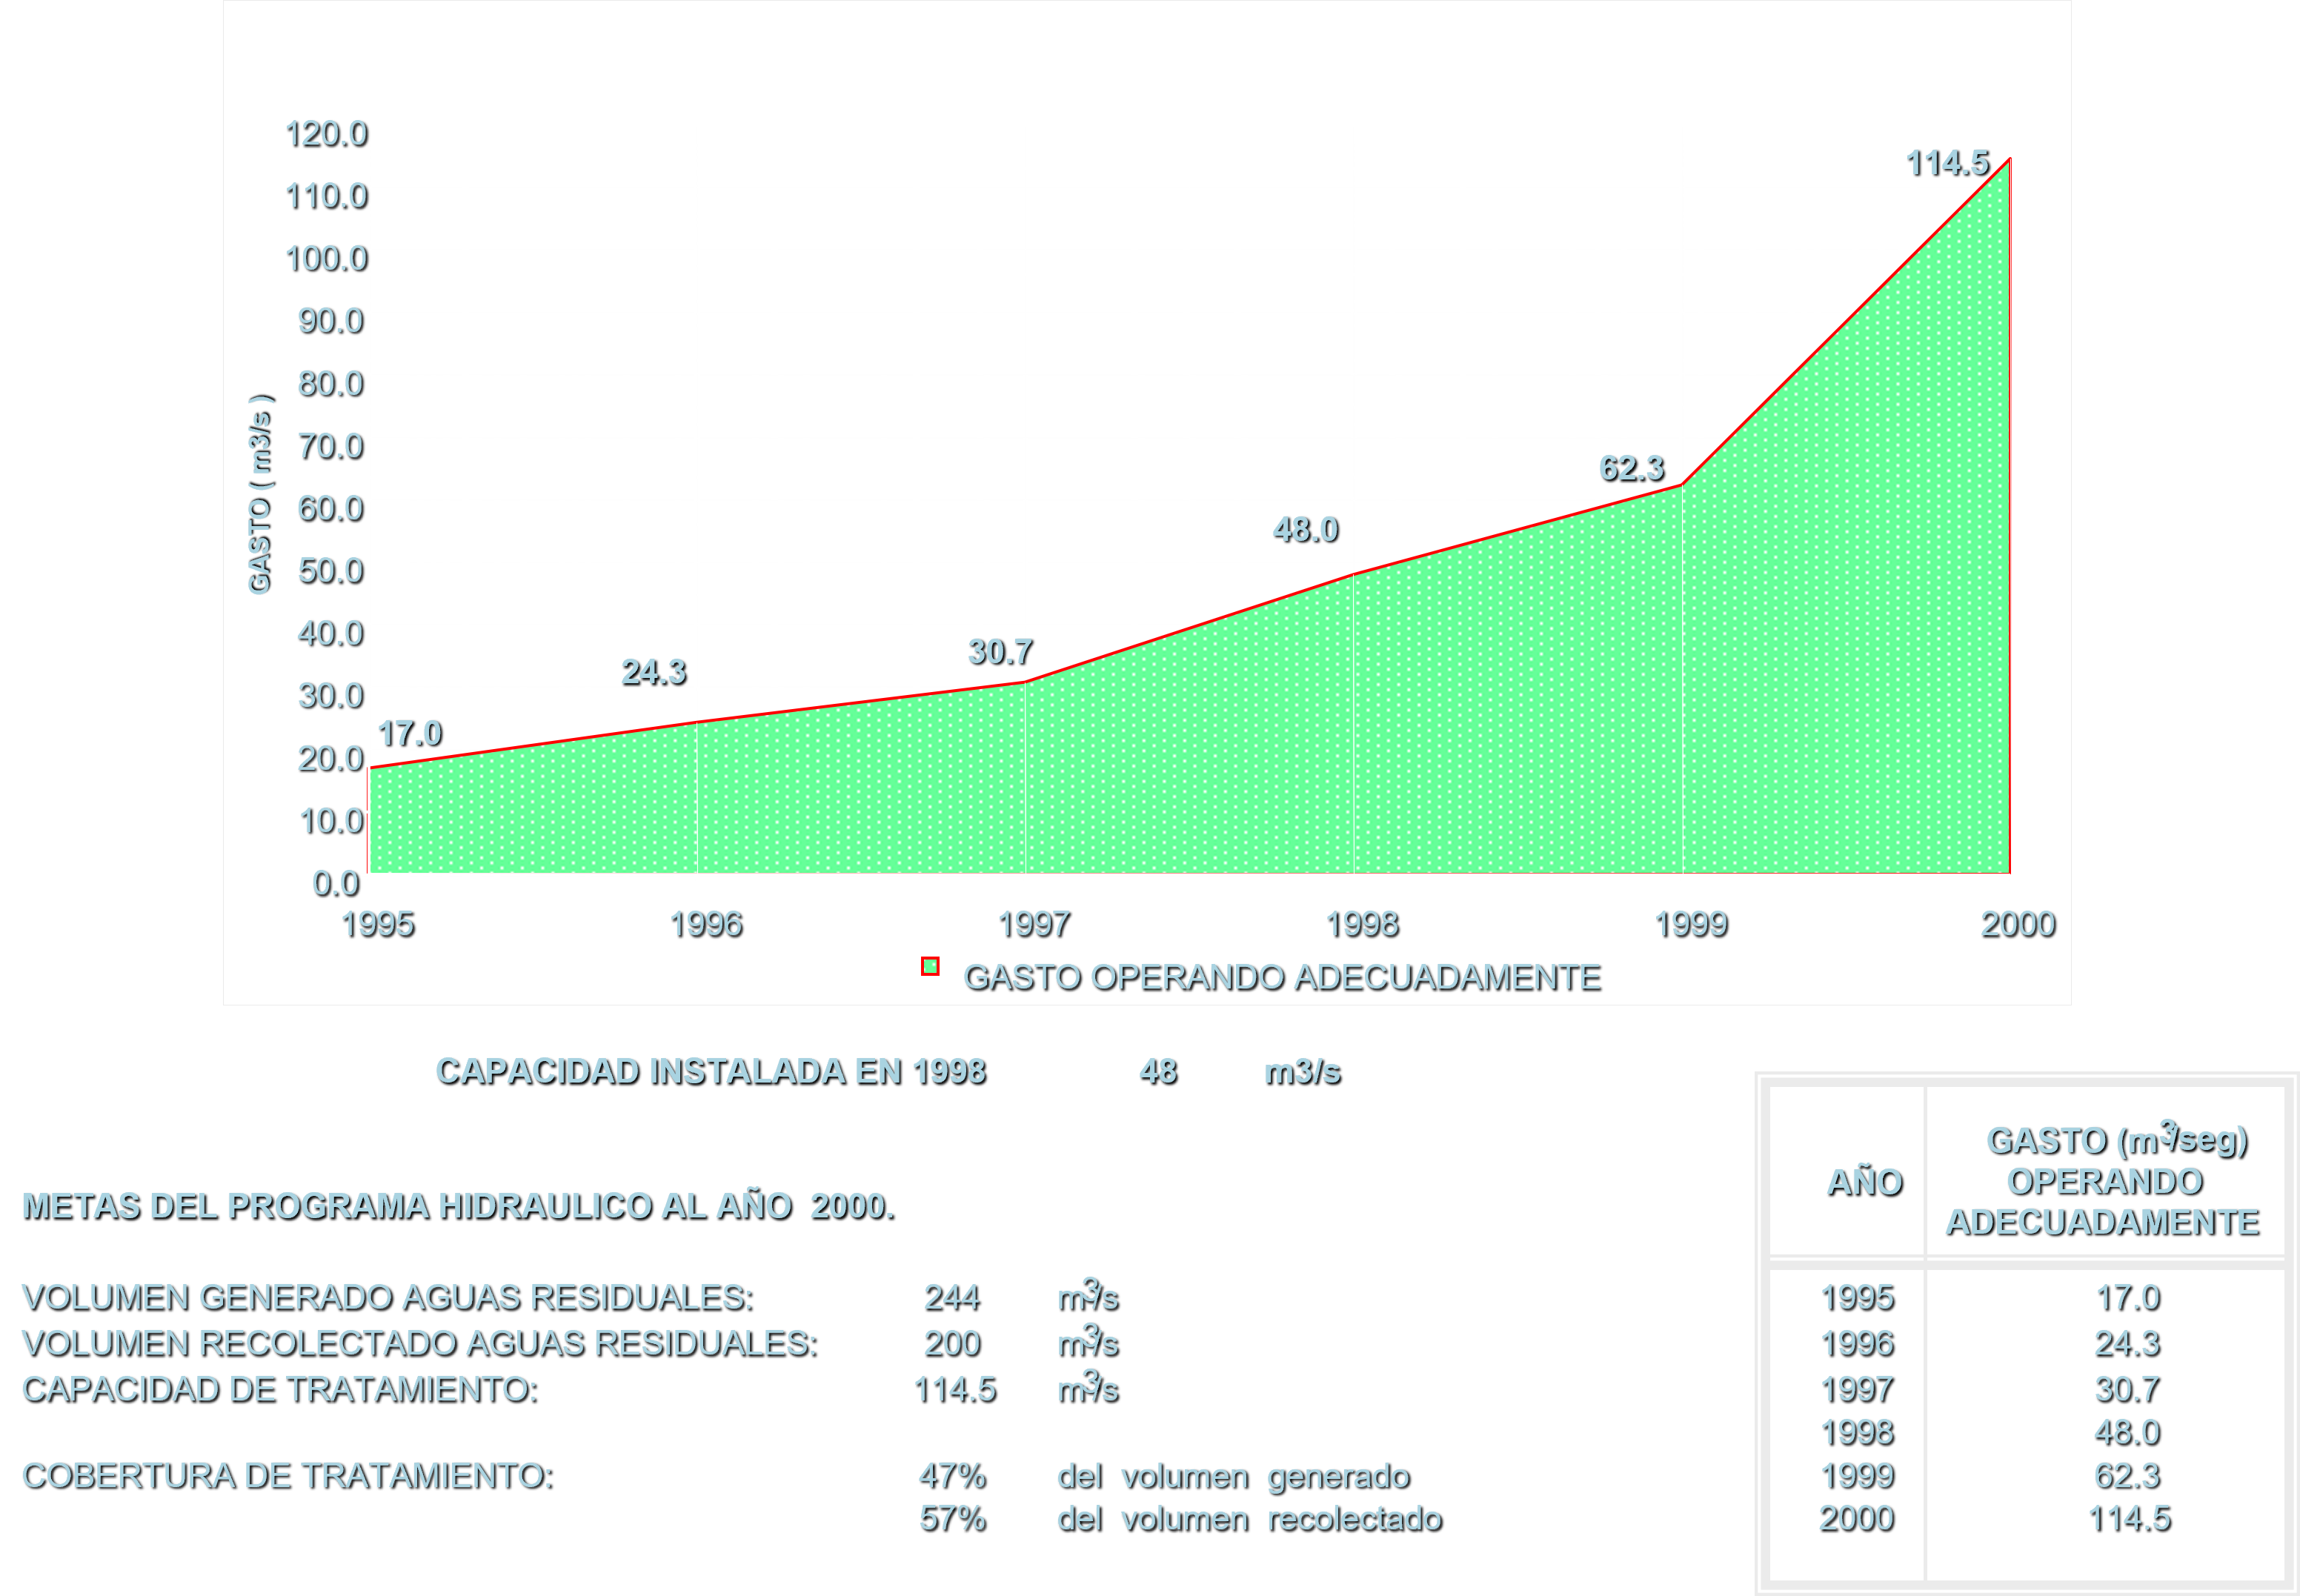
\includegraphics[width=0.5\textwidth]{ar1.png}
  \caption{Cobertura de saneamiento 1995 - 2000\cite{cruz2013precio}}
  \label{ar1}
\end{figure}
\begin{table}[h!]
    \centering
    \begin{tabular}{@{}|c|ccccc|@{}}
    \toprule
    \multirow{2}{*}{Tipo de Reuso} &
      \multicolumn{5}{c|}{Promedio Mensual} \\ \cmidrule(l){2-6} 
     &
      \multicolumn{1}{c|}{\begin{tabular}[c]{@{}c@{}}Coliformes   Fecales\\ NMP/100   ml\end{tabular}} &
      \multicolumn{1}{c|}{\begin{tabular}[c]{@{}c@{}}Huevos   de\\ Helmintos\\ (h/l)\end{tabular}} &
      \multicolumn{1}{c|}{\begin{tabular}[c]{@{}c@{}}Grasas   y\\ Aceites\\ mg/l\end{tabular}} &
      \multicolumn{1}{c|}{DBO5   mg/l} &
      SST   mg/l \\ \midrule
    \begin{tabular}[c]{@{}c@{}}Servicios al \\ público con\\ contacto directo\end{tabular} &
      \multicolumn{1}{c|}{240} &
      \multicolumn{1}{c|}{$\geq 1$} &
      \multicolumn{1}{c|}{15} &
      \multicolumn{1}{c|}{20} &
      20 \\ \midrule
    \begin{tabular}[c]{@{}c@{}}Servicios al\\ público con \\ contacto directo\\ u ocasional\end{tabular} &
      \multicolumn{1}{c|}{1,000} &
      \multicolumn{1}{c|}{$\geq 5$} &
      \multicolumn{1}{c|}{15} &
      \multicolumn{1}{c|}{30} &
      30 \\ \bottomrule
    \end{tabular}
    \caption{Límites máximos permisibles de contaminantes NOM-003-ECOL-1997\cite{las1973norma}}
    \label{tabar2}
\end{table}
\begin{table}[h!]
    \centering
    \begin{tabular}{@{}ccc@{}}
    \toprule
    Parámetro        & Unidad       & Criterio de calidad \\ \midrule
    Col. Fecales     & NMP/100   ml & 200                 \\
    Col. Totales     & NMP/100   ml & 1000                \\
    DBO5   Total     & mg/l         & 20                  \\
    DQO Total        & mg/l         & 50                  \\
    Grasas y Aceites & mg/l         & 5                   \\
    SAAM             & mg/l         & 1                   \\ \bottomrule
    \end{tabular}
    \caption{Criterios de calidad en el reuso de agua renovada\cite{cortes1997reuso}}
    \label{tabra3}
\end{table}
\subsection{Aguas residuales}
Son líquidos de composición variada provenientes de los usos domésticos, de fraccionamiento agropecuario, industrial, comercial, de servicios o de cualquier otro uso, que por estos sufran una degradación de su calidad original.
\subsubsection{Tratamiento y composición}
El tratamiento es un proceso natural o artificial que consiste en remover o alterar por métodos físicos, químicos y biológicos, las materias en suspensión, coloidales y disueltas de las aguas residuales convirtiéndolas en aguas menos nocivas o peligrosas.
\begin{table}[h!]
    \centering
    \begin{tabular}{@{}cc@{}}
    \toprule
    Orgánicos &
      Inorgánicos \\ \midrule
    \begin{tabular}[c]{@{}c@{}}Materia orgánica\\ Biológicos\\ Microbianos   \\ Hidrocarburos \\ Pesticidas\\ Detergentes\end{tabular} &
      \begin{tabular}[c]{@{}c@{}}Radioactivos   \\ Térmicos\\ Metálicos\\ No   metálicos\end{tabular} \\ \bottomrule
    \end{tabular}
    \caption{Clasificación de los tipos de contaminates\cite{arana1996tratamiento}}
    \label{tabar4}
\end{table}
\begin{itemize}
    \item Métodos de evaluación para la demanda de oxígeno (DTeO, DQO, DBO y DTO).
    \item Métodos  para la evaluación de parámetros de contenido en carbono (COTe y COT).    
\end{itemize}
\subsection{Métodos de tratamiento de Aguas Residuales}
\begin{itemize}
    \item Pretratamiento
    \item Tratamiento primario
    \item Tratamiento secundario
    \item Tratamiento terciario
\end{itemize}
\begin{definition}[Planta de tratamiento]
    A manera de descripción una planta de tratamiento esta integrada de una serie de unidades que realizan un proceso físico-químico y/o biológico, ya sea de agua blanca o agua residual.
\end{definition}
Dentro de la información requerida para el proyecto de una planta de tratamiento como la selección del método tenemos:
\begin{enumerate}
    \item Determinar la naturaleza del agua residual.
	\item Evaluación de la carga contaminante.
	\item Calidad del efluente requerido.
	\item Estimación del gasto de diseño.
	\item Costo y disponibilidad del terreno.
	\item ampliaciones futuras y/o posibles modificaciones de las normas ecológicas.
\end{enumerate}

Porcentaje calculado con respecto a las 1018 plantas de tratamiento construidas.
\begin{figure}[h!]
\centering
  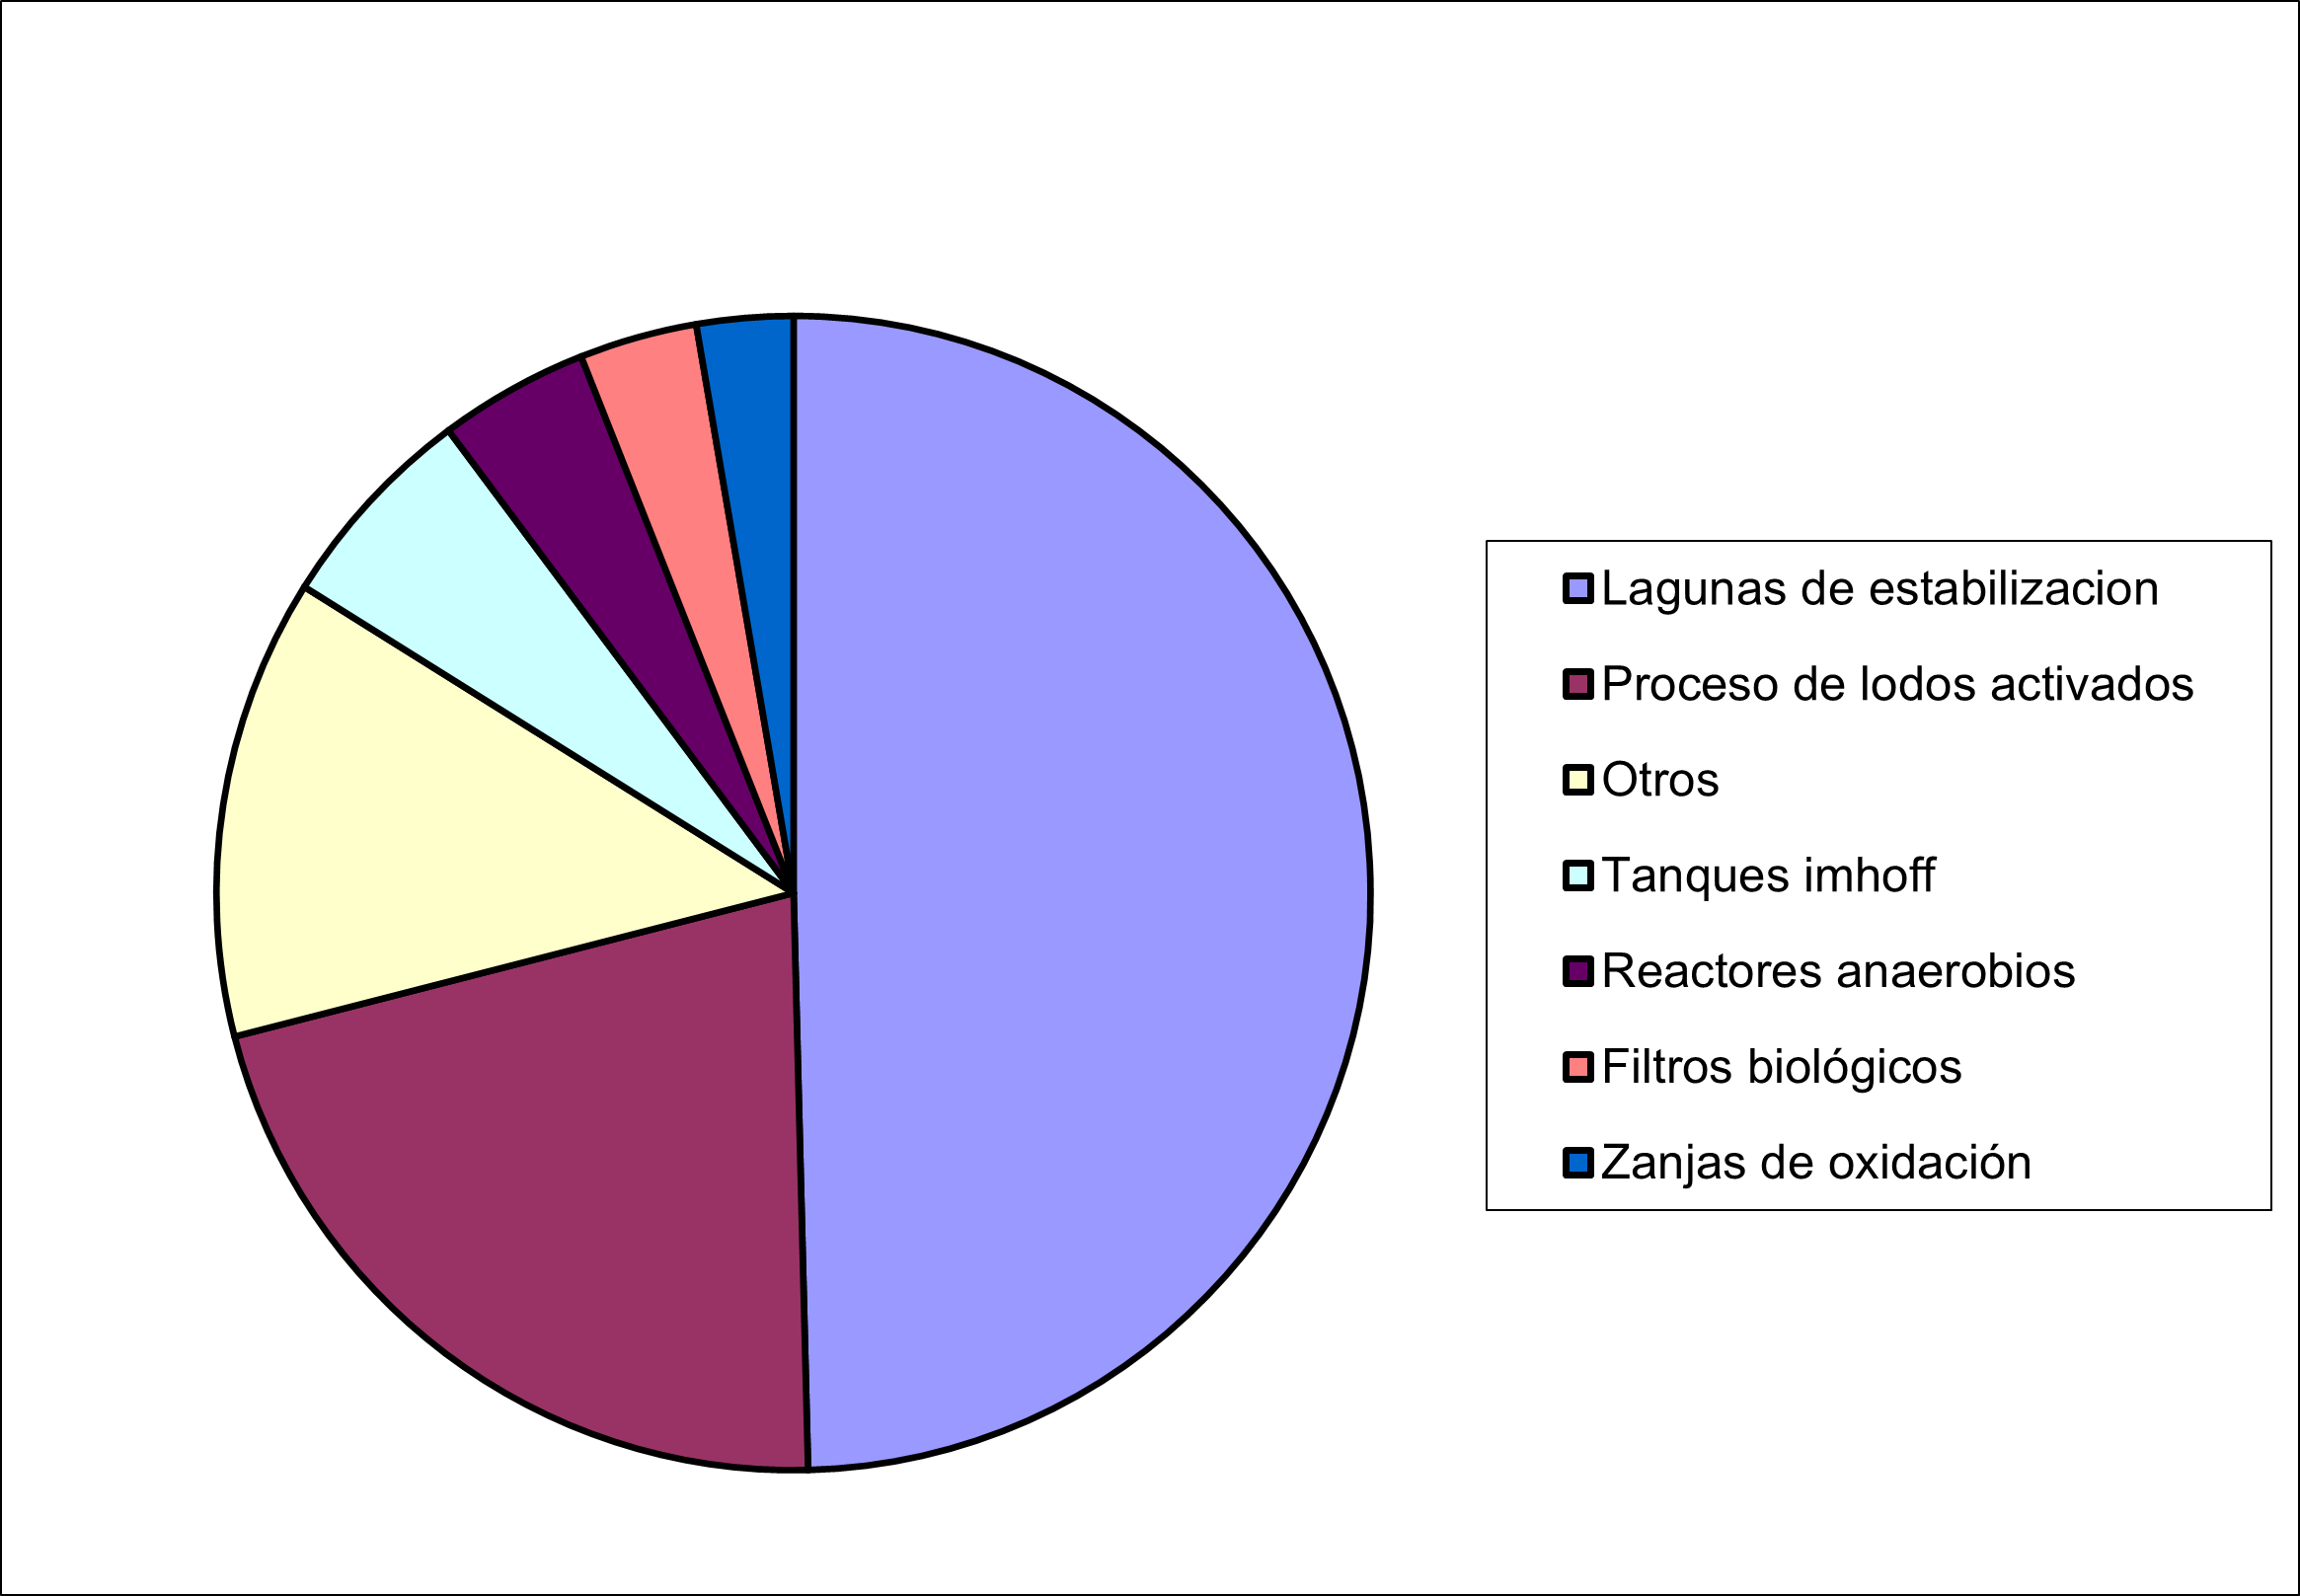
\includegraphics[width=0.5\textwidth]{ar2.png}
  \caption{Porcentaje calculado con respecto a las 1018 plantas de tratamiento construidas}
  \label{ar2}
\end{figure}
\begin{definition}[Rejas]
    Su objetivo es la retención de sólidos gruesos presentes en el agua residual, a fin de proteger los equipos de las plantas de tratamiento (bombas, válvulas, líneas de conducción, etc.) contra posibles daños y obstrucciones, véase la figura \ref{ar5}.
\end{definition}
\begin{figure}[h!]
\centering
  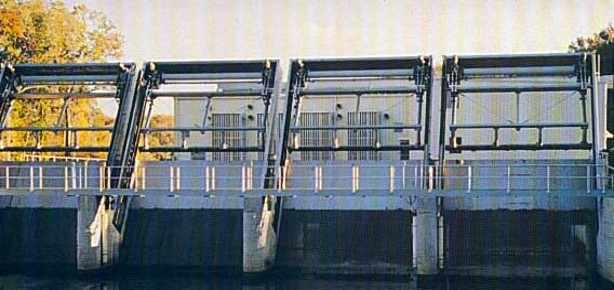
\includegraphics[width=0.5\textwidth]{ar5.jpg}
  \caption{Rejas}
  \label{ar5}
\end{figure}
\begin{figure}[h!]
\centering
  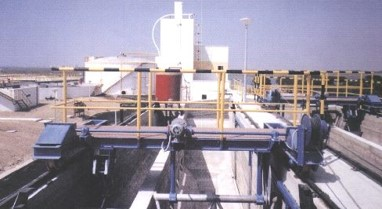
\includegraphics[width=0.5\textwidth]{ar3.jpg}
  \caption{Sistemas de extracción de arenas Puente barredor desengrasador de arenas ''Accionamiento alternativo}
  \label{ar3}
\end{figure}

\begin{figure}[h!]
\centering
  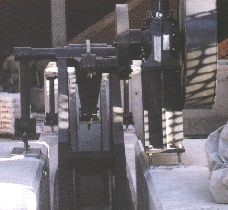
\includegraphics[width=0.5\textwidth]{ar4.jpg}
  \caption{Tanques separadores de grasas}
  \label{ar4}
\end{figure}
Su objetivo es la separación del agua residual de sustancias más ligeras que el agua que de forma natural o inducida tienden a flotar.

De acuerdo a los mecanismos empleados para la separación de estas sustancias se pueden clasificar en:
\begin{itemize}
    \item Flotación por Gravedad
    \item Flotación Inducida por Aire    
\end{itemize}

\subsubsection{Tratamiento Primario}
El tratamiento primario elimina entre un 90 y 95\% de los sólidos sedimentables

Los residuos sólidos recolectados en el fondo se llaman lodos residuales. En esta fase se denominan lodos primarios. En cuanto a los sólidos en suspensión, del 40 al 60% se eliminan en el proceso de sedimentación al que a veces se añaden floculantes.

\subsubsection{Tratamiento Secundario}
Tratamientos secundarios más importantes
\begin{itemize}
    \item Fangos activados
    \item Filtros percoladores
    \item Biodiscos (CBRS)
    \item Lagunas de oxidación
\end{itemize}
\begin{figure}[h!]
\centering
  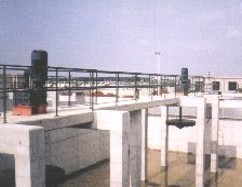
\includegraphics[width=0.5\textwidth]{ar6.jpg}
  \caption{Turbinas de aireación}
  \label{ar6}
\end{figure}

\begin{definition}[Filtros percoladores]
    Los filtros de goteo son el segundo método más utilizado de tratamiento secundario. En este método las aguas residuales se pulverizan sobre un lecho de piedras o trozos de plástico moldeados.
\end{definition}
\begin{figure}[h!]
\centering
  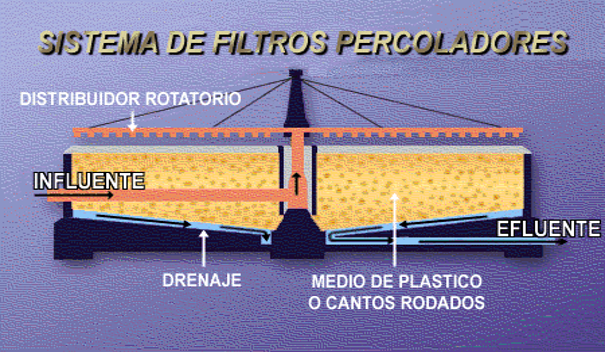
\includegraphics[width=0.5\textwidth]{ar7.png}
  \caption{Filtros Percoladores}
  \label{ar7}
\end{figure}
\begin{definition}[Biodiscos]
    El efluente de un CBR continúa hacia el clarificador secundario donde la biomasa, que se ha desprendido del medio filtrante sedimenta. El sedimento se bombea hacia las instalaciones para el tratamiento de sólidos o hacia el clarificador primario
\end{definition}
\begin{figure}[h!]
\centering
  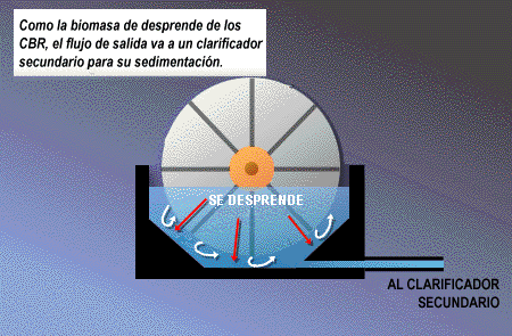
\includegraphics[width=0.5\textwidth]{ar8.png}
  \caption{Biodiscos}
  \label{ar8}
\end{figure}
\begin{definition}[Lagunas de oxidación]
    Su diseño varía pero, en general, están organizadas en dos fases. En la primera fase, la laguna es tan profunda que las condiciones son casi completamente anaeróbicas . En esta fase sedimentan los lodos. La segunda fase consiste en una laguna o serie de lagunas poco profundas donde ocurren reacciones microbianas aerobias
\end{definition}
\begin{figure}[h!]
\centering
  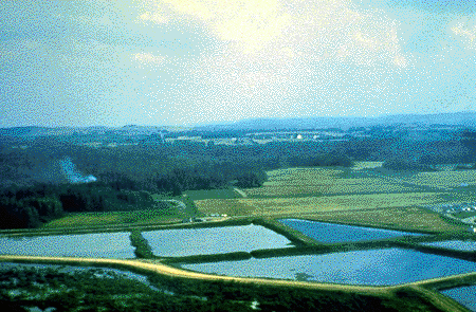
\includegraphics[width=0.5\textwidth]{ar9.png}
  \caption{Lagunas de oxidación}
  \label{ar9}
\end{figure}
\begin{figure}[h!]
\centering
  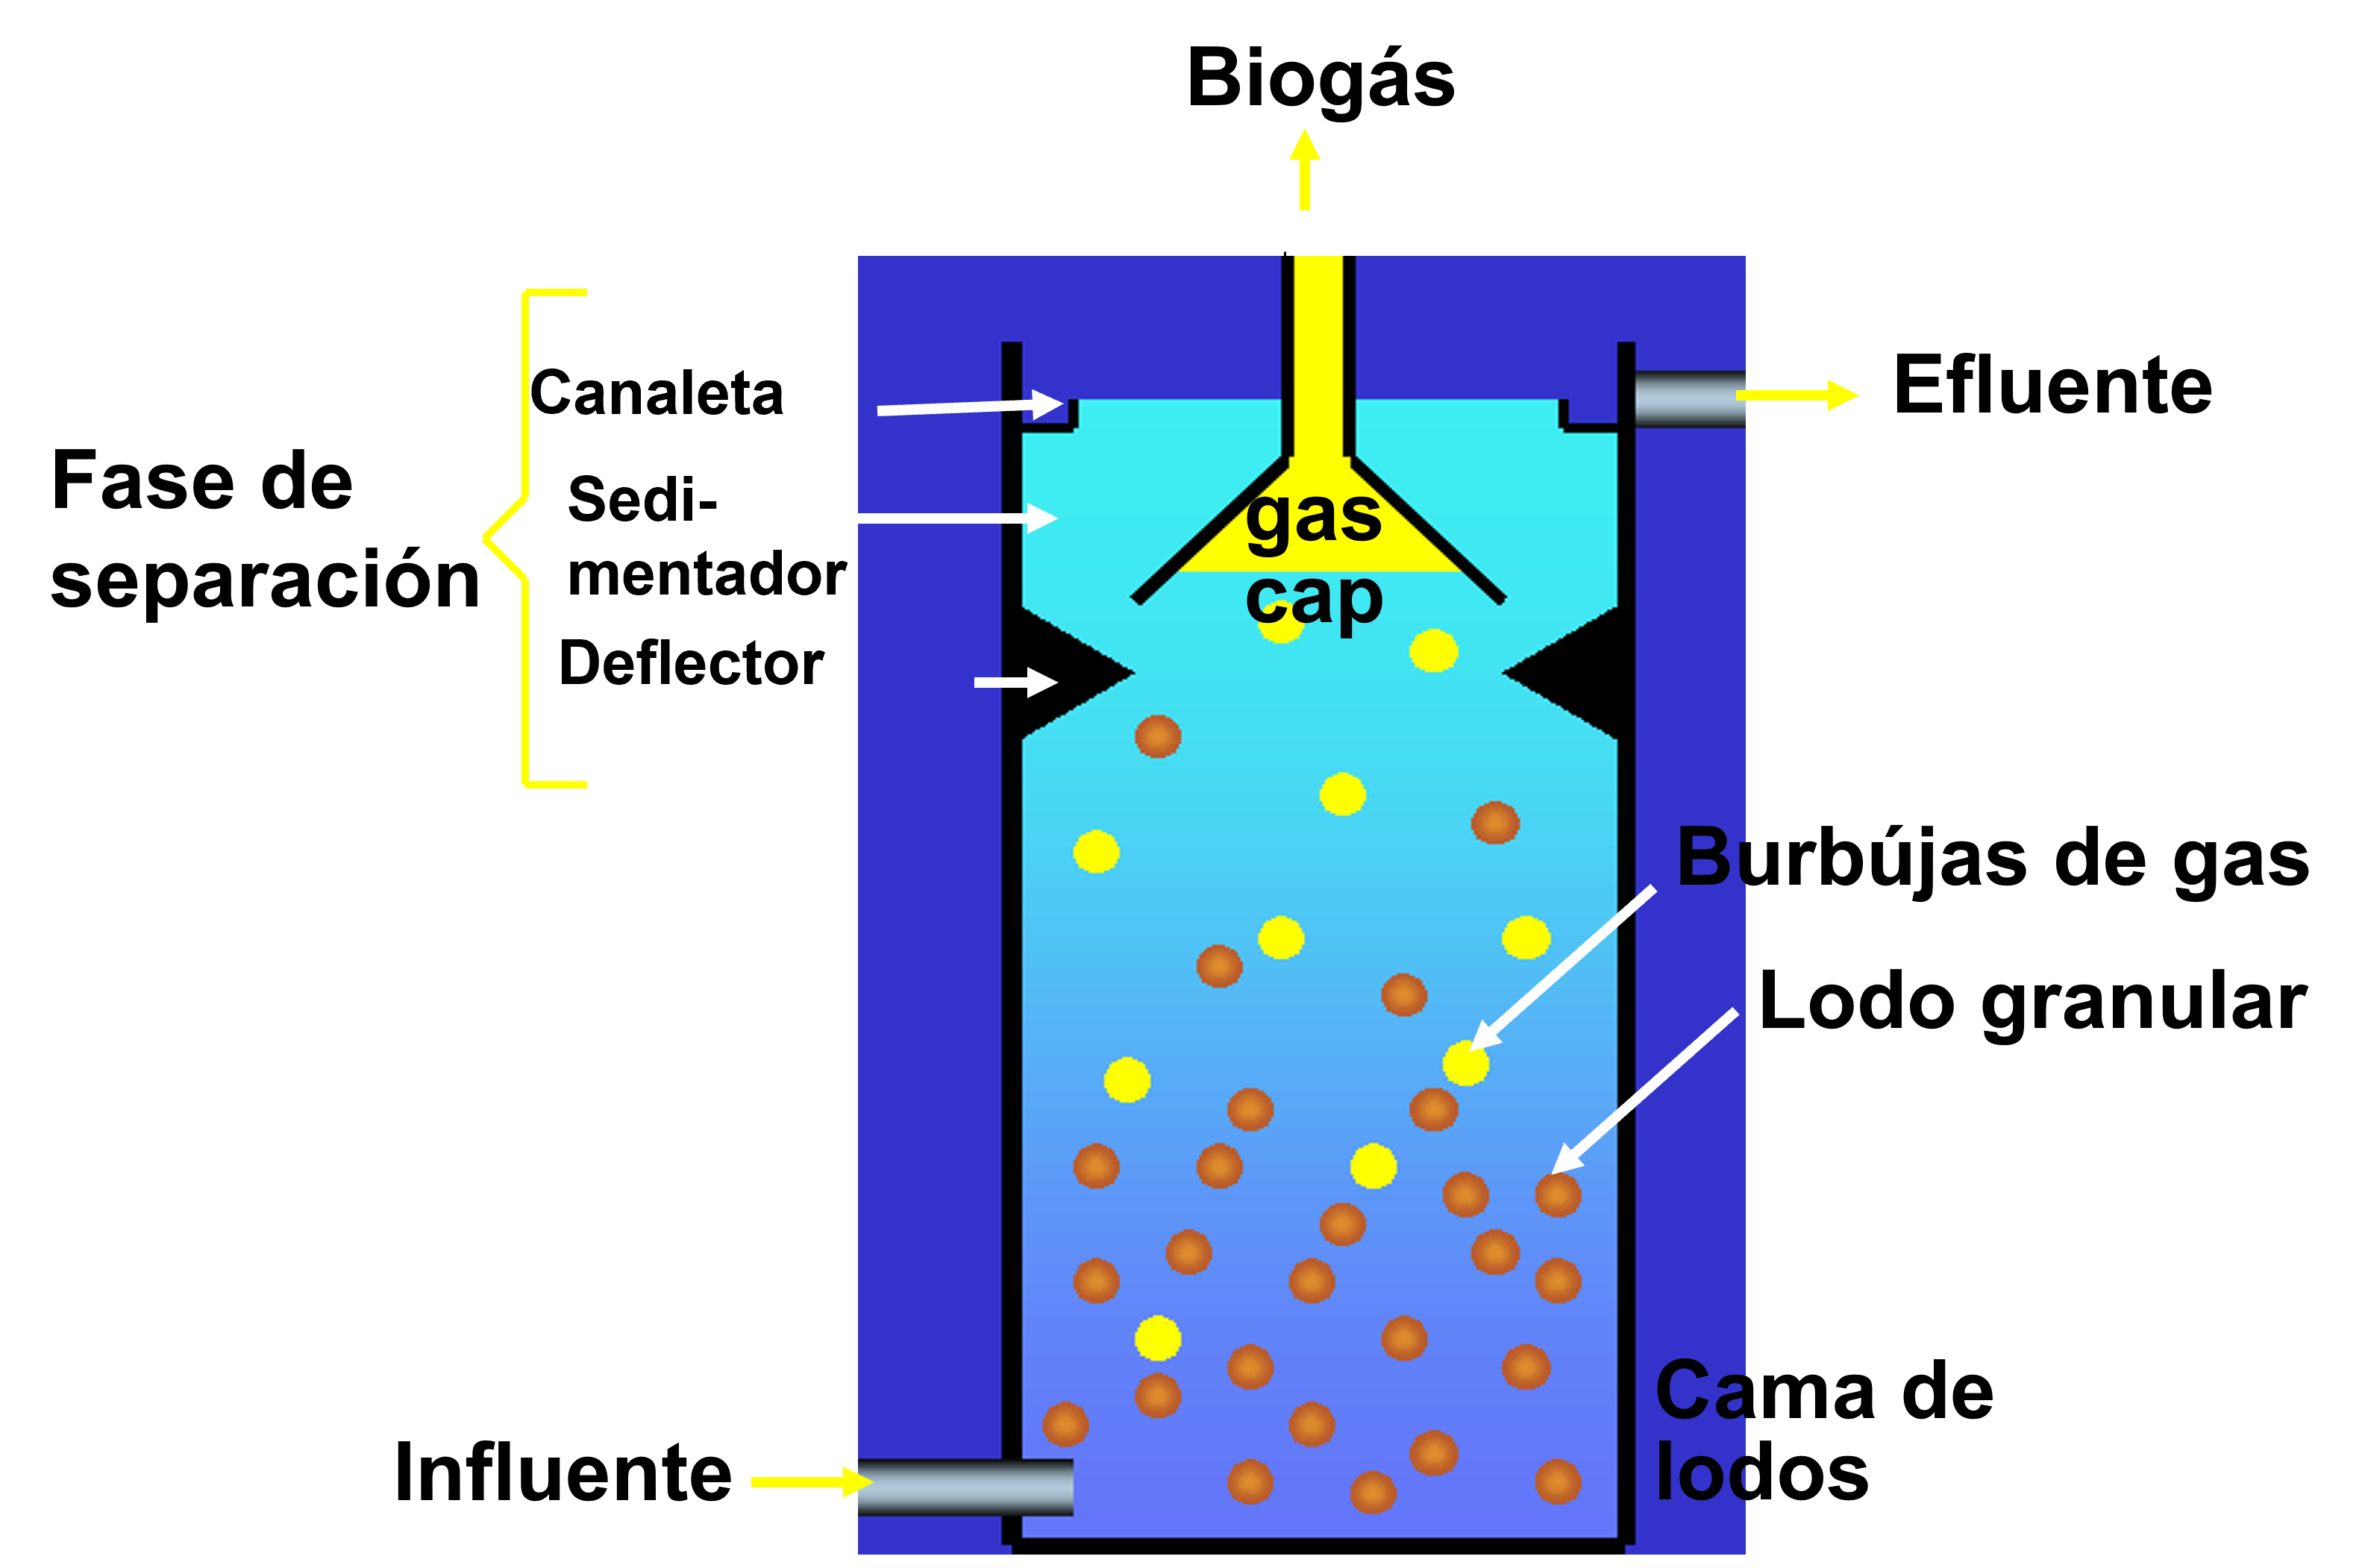
\includegraphics[width=0.5\textwidth]{ar10.png}
  \caption{Reactor UASB}
  \label{ar10}
\end{figure}
% TODO: MAPA CONCEPTUAL QUE ME DA HUEVA PONER EN FIGMA

\subsection{Digestión anaerobia}
El tratamiento anaerobio se utiliza tanto para las aguas residuales como para la digestión de los lodos. Los productos finales de la degradación anaerobia son gases, principalmente metano $(CH_4)$, dióxido de carbono $(CO_2)$ y pequeñas cantidades de sulfuro de hidrogeno $(H_2S)$, mercaptano $(RSH)$ e hidrogeno $(H_2)$. El proceso comprende dos etapas: (A) fermentación ácida y (B) fermentación metánica.
% \schemestart CH_3COOH \arrow{->} CO_2+CH_4 \schemestop\par 

% \schemestart
% \chemname{\chemfig{R-C(-[:-30]OH)=[:30]O}}{Carboxilic\\Acid}
% \+
% \chemname{\chemfig{R’OH}}{Alcohol}
% \arrow(.mid east--.mid west)
% \chemname{\chemfig{R-C(-[:-30]OR’)=[:30]O}}{Ester}
% \+
% \chemname{\chemfig{H_2O}}{Water}
% \schemestop
% \chemnameinit{}

\subsection{Efecto de la Aplicación de Aguas Residuales en el Suelo,en Cultivos y en Hombre}

\subsubsection{Efectos en propiedades físicas del suelo}
\begin{itemize}
    \item Incrementa en contenido de humus
    \item Mejora la estructura
    \item Reduce riesgos de erosión 
    \item Incrementa la capacidad para retener humedad. 
    \item Otro cambio favorable es el incremento en espacio poroso del suelo.
    \item Pero el exceso de materiales orgánicos agregados al suelo, causa problemas de drenaje (colores grises) que afectan el crecimiento de plantas y las condiciones de aireación.    
\end{itemize}
\subsubsection{Efectos en propiedades químicas del suelo}
En contraste con las propiedades físicas, son considerables debido a la aplicación de las aguas residuales. Por ejemplo: El K, Ca, Mg, Na. La elevada concentración de Na y otros cationes ocasiona una elevada acumulación de sales en los terrenos irrigados con el agua residual. 
El incremento en materia orgánica del suelo contribuye con cargas adicionales para la retención de cationes, mejorando con ello la CIC.

El uso de grandes cantidades de aguas residuales en terrenos puede degradar el suelo, el agua y el aire. 
Sus subproductos, componentes o productos pueden causar problemas de olores, liberar gases a la atmósfera o contaminar el suelo y el agua con nutrientes, elementos tóxicos y microorganismos 

\subsubsection{Daños de los detergentes a las plantas}
Aseguran que el ABS indica daños en las plantas tales como inhibición del crecimiento, pérdida de clorofila (hojas cloróticas), alteración de la germinación sobre los productores primarios (fitoplancton) especialmente las algas \cite{streitwieser1963isotope}, dilación del crecimiento, penetración de los detergentes en las células ocasionando citólisis del núcleo, inactivación de las enzimas y efectos secundarios.

Alto. Infecciones intestinales originadas por nemátodos como: Ascaris, Trichuris y Uncinaria.
Menor. Infecciones bacterianas tales  como: diarreas bacterianas por ejemplo: cólera y tifoidea
Mínimo. Infecciones virales excretadas como: diarreas excretadas por rotavirus y la hepatitis A.
Entre alto y nulo, dependiendo de la práctica particular en la utilización de excretas y de las circunstancias locales. Infecciones provocadas por tremátodos y cestos, algunos ejemplos son: esquistosomiasis, clonorquiasis y teniasis.
\begin{table}[h!]
    \centering
    \begin{tabular}{@{}ccc@{}}
    \toprule
    \multicolumn{3}{c}{EFECTOS   CAUSADOS POR COMPUESTOS QUE SE ENCUENTRAN EN AGUA CONTAMINADA} \\ \midrule
    Compuestos &
      Fuente &
      Efectos   sobre la Salud \\
    Nitratos   y Nitritos &
      \begin{tabular}[c]{@{}c@{}}Natural:Solubilización\\ de rocas. Artificial: \\ Practicas agrícolas\\ como: abonado\\ o contaminación por\\ aguas residuales.\end{tabular} &
      \begin{tabular}[c]{@{}c@{}}Su   presencia en concentraciones de mg/l provoca\\  metahemoglobinemia infantil,   sobre todo en lactantes\\ (nitratos). Se pueden combinar con amidas secundarias\\ de origen alimentarlo las cuales tienen poder cancerígeno.\end{tabular} \\
    Fluoruros &
       &
      \begin{tabular}[c]{@{}c@{}}Ocasionan   la florosis y ostioflorosis. Disminución \\ de caries hasta en un 70\%\end{tabular} \\
    Sulfatos &
      \begin{tabular}[c]{@{}c@{}}Su   procedencia\\ es similar a la de\\ los cloruros\end{tabular} &
      \begin{tabular}[c]{@{}c@{}}En cantidades elevadas ocasiona transtornos\\ gastrointestinales en niños\end{tabular} \\
    Yodo &
       &
      Su carencia origina el bocio andémico \\
    Fenoles &
      \begin{tabular}[c]{@{}c@{}}Procesos   industriales,    \\ como: industrias\\ colorantes, papeleras\end{tabular} &
      \begin{tabular}[c]{@{}c@{}}A concentraciones de 0.01 ppm y en combinación con el\\ cloro producen   clorofenoles, que dan al agua en sabor\\ medicamentoso muy fuerte\end{tabular} \\
    Haloformos &
      \begin{tabular}[c]{@{}c@{}}Cloración   de aguas para\\ beber que contengan \\ acido húmico y fúlvico,\\ que da origen \\ a trihalometanos\end{tabular} &
      \begin{tabular}[c]{@{}c@{}}Los   trihalometanos tienen poder \\ cancerigeno experimental\end{tabular} \\ \bottomrule
    \end{tabular}
    \caption{Efectos en la salud causados por elementos y/o compuestos}
    \label{tabmar1}
\end{table}
En los cultivos para consumo humano directo se debe suspender el riego 30 días antes de la cosecha y tomar medidas de desinfección en los cultivos que se consumen crudos.
En cuanto a salinidad (suelos), hacer lavados. En cuanto al boro se puede utilizar agua negra para cultivos semitolerantes y tolerantes.

\subsection{Métodos de riego con aguas residuales}
Las aguas residuales constituyen un problema sanitario, pero a su vez un recurso muy apreciado para el riego y la piscicultura; de gran valor económico en áreas desérticas o con estiajes prolongados. 
Los nutrientes presentes en las aguas residuales tienen valor como fertilizantes y aumentan el rendimiento de los cultivos, estos nutrientes se conservan en el protoplasma de las algas al tratar las aguas residuales en lagunas de estabilización. 
\begin{itemize}
    \item \textbf{Por anegamiento (método de riego por inundación)}: de esta forma se humedece casi toda la superficie del terreno
    \item \textbf{En surcos}: sólo se humedece parte de la superficie del suelo
    \item \textbf{El anegamiento}: demanda la menor inversión, pero quizá expone a los agricultores al mayor peligro.
    \item \textbf{El riego por aspersión}: No es conveniente para las verduras ni las frutas a menos que el efluente se ajuste a las condiciones estipuladas en las directrices correspondientes y las verduras no se deben regar por anegamiento.
    \item \textbf{Riego localizado}:  (en pequeños chorros, por goteo o en burbujas); se humedece gradualmente la zona de la raíz de cada planta
    \item \textbf{El riego del subsuelo o el localizado}: sobre todo cuando se coloca en la superficie una cubierta plástica (vegetal) protectora, puede ofrecer el mayor grado de protección de la salud, además de permitir un uso más eficiente del agua y dar mayores rendimientos. Sin embargo, es costoso y se necesita un tratamiento seguro y completo del agua.
\end{itemize}
Tratar de eliminar las posibles molestias causadas por moscas, mosquitos, olores, etc.

Salud ocupacional: Proteger la salud de los campesinos. Si el clima y las circunstancias lo permiten, considerar el uso de guantes, botas, etc. Debe existir control médico (Chequeo cada 3 meses) del personal y de sus familiares que vivan en el área de riego. 

Deberá hacerse un monitoreo sobre calidad toxicológica y microbiológica de los productos procedentes de estas áreas de riego. Como patrón de comparación deberá hacerse el mismo tipo de control con productos procedentes de áreas de riego donde no se utilicen aguas residuales o altamente contaminadas. 

\subsubsection{Obstrucción de emisores en el riego localizado y por Aspersión}

Uno de los principales problemas del empleo de aguas residuales en riego localizado (goteo o micro-aspersión) es la obturación de los emisores por los sólidos en suspensión de estas aguas. En general, la cloración y un buen filtrado resuelven estos problemas. 

Hay que filtrar el agua residual en los Sistemas de riego por escorrentía y a través de canales o surcos, camellones y surcos para evitar la inundación de los cultivos. 

El alto contenido de sales que se le aplica la suelo si esta no es bien tratada provoca salinización en los suelos

El impacto de las aguas negras o residuales en los recursos naturales tales como flora y fauna silvestre, fuentes de agua, aire, suelos y en la salud humana es un asunto de interés mundial que toma una preocupación creciente debido a la necesidad de reusar el agua en diferentes actividades del quehacer humano.

En México se cuenta con unas 1150 plantas de tratamiento de aguas residuales municipales, con una capacidad instalada total demás de 80,000 l/s y un caudal tratado de 51,000 l/s, mientras que la capacidad instalada de plantas industriales es de 42,000 l/s y un caudal tratado de 25,000 l/s. 
\begin{longtable}[c]{@{}ccccc@{}}
    \toprule
    Grupo &
      Agente &
      Frecuencia &
      Vía de Acceso &
      Enfermedad \\* \midrule
    \endhead
    %
    \bottomrule
    \endfoot
    %
    \endlastfoot
    %
    \multirow{3}{*}{Virus} &
      \begin{tabular}[c]{@{}c@{}}Virus de la\\ Hepat. A. Epidém\\ Caxsachie\end{tabular} &
      \dots &
      Oral &
      \begin{tabular}[c]{@{}c@{}}H. Epidémica\\ Indecciones Gastro-\\ intestinales\end{tabular} \\
     &
      Adenovirus &
      \dots &
      \begin{tabular}[c]{@{}c@{}}Cutáneo\\ Mucosa\\ (Contacto)\end{tabular} &
      \begin{tabular}[c]{@{}c@{}}Conjutivitis de\\ las piscinas\end{tabular} \\
     &
      \begin{tabular}[c]{@{}c@{}}Polimielíticos\\ Echovirus\end{tabular} &
      $\cdot\cdot$ &
      Oral &
      \begin{tabular}[c]{@{}c@{}}Parálisis\\ Afecciones diversas\end{tabular} \\
    \multirow{3}{*}{Bacterias} &
      \begin{tabular}[c]{@{}c@{}}Salmonella typhy\\ Salmonella paratyphu\\ Shigella disenteriae\end{tabular} &
      \dots &
      Oral &
      \begin{tabular}[c]{@{}c@{}}Fiebre Tifoidea\\ Fiebre Paratífica\\ Disentería Bacilar\end{tabular} \\
     &
      \begin{tabular}[c]{@{}c@{}}Pasteurella tularensis\\ Leptosperia\\ Eschericia Coli\\ Enteropatógena\end{tabular} &
      $\cdot\cdot$ &
      Oral &
      \begin{tabular}[c]{@{}c@{}}Tularemia\\ Leptospirosis\\ Colitis a recién\\ nacidos\end{tabular} \\
     &
      \begin{tabular}[c]{@{}c@{}}Bacillus anthracis\\ Brucellas\\ Lectospiras\end{tabular} &
      $\cdot\cdot$ &
      Cutáneo-Mucosa &
      \begin{tabular}[c]{@{}c@{}}Carbunco\\ Fiebre de Malta\\ Afecciones icte-\\ rohemorrágicas\end{tabular} \\
    \multirow{2}{*}{Protozoos} &
      \begin{tabular}[c]{@{}c@{}}Entomoeba histolytica\\ Balantidium coli\\ Leishmanias\\ Giardia Lamblia\end{tabular} &
      \begin{tabular}[c]{@{}c@{}}\dots\\ $\cdot\cdot$\end{tabular} &
      \begin{tabular}[c]{@{}c@{}}Oral\\ Oral\end{tabular} &
      \begin{tabular}[c]{@{}c@{}}Disentería Amebiana\\ Balantidiasis\\ Leishmaniasis\\ Lambliasis\end{tabular} \\
     &
      Leishmanias &
      $\cdot$ &
      Oral &
      Leishmaniasis \\
    \multirow{2}{*}{Ritcketsiales} &
      Chalmydia &
      \dots &
      \begin{tabular}[c]{@{}c@{}}Cutáneo\\ Mucosa\\ (contacto)\end{tabular} &
      \begin{tabular}[c]{@{}c@{}}Conjuntivitis\\ oculo-genitales\\ de\\ inclusión\end{tabular} \\
     &
      Chalmydozoon trachomatis &
      $\cdot\cdot$ &
      \begin{tabular}[c]{@{}c@{}}Cutáneo\\ Mucosa\end{tabular} &
      Tracoma \\
    \begin{tabular}[c]{@{}c@{}}Gusanos\\ (Cercarias)\end{tabular} &
      \begin{tabular}[c]{@{}c@{}}Shistosomas\\ \\ \\ Fasciola hepática\\ Dracuncula medinensis\end{tabular} &
      \dots &
      \begin{tabular}[c]{@{}c@{}}Cutáneo\\ Mucosa\\ (contacto)\end{tabular} &
      \begin{tabular}[c]{@{}c@{}}Schistosomiasis\\ en países tropicales\\ \\ Distomatosis\\ Dracunculosis\end{tabular} \\
    \begin{tabular}[c]{@{}c@{}}Gusanos\\ (huevos)\end{tabular} &
      \begin{tabular}[c]{@{}c@{}}Ascaris\\ Tenia equinococo\end{tabular} &
      $\cdot\cdot$ &
      Oral &
      \begin{tabular}[c]{@{}c@{}}Ascaridiasis\\ Hidatosis\end{tabular} \\* \bottomrule
    \caption{Enfermedades Causadas por Agentes Patógenos que pueden estar contenidos en el Agua}
    \label{tabmar2}\\
\end{longtable}
\begin{definition}[Metales pesados]
    Son aquellos cuya densidad es por lo menos cinco veces mayor que la del agua. Tienen aplicación directa en numerosos procesos de producción de bienes y servicios. Los más importantes son: 
	Arsénico (As), Cadmio (Cd), Cobalto (Co), Cromo (Cr), Cobre (Cu), Mercurio (Hg), Níquel (Ni), Plomo (Pb), Estaño (Sn) y  Cinc (Zn).
\end{definition}
\begin{table}[h!]
    \centering
    \begin{tabular}{@{}cccccc@{}}
    \toprule
    METAL &
      \multicolumn{2}{c}{\begin{tabular}[c]{@{}c@{}}CONCENTRACIÓN\\ EN SUELOS\end{tabular}} &
      \multicolumn{2}{c}{\begin{tabular}[c]{@{}c@{}}CONCENTRACIÓN\\ EN LODOS\end{tabular}} &
      \begin{tabular}[c]{@{}c@{}}CARGA\\ MÁXIMA\end{tabular} \\ \midrule
           & pH   suelo <7 & pH   suelo >7 & pH   suelo <7 & pH   suelo >7 & (a 10 años) \\
    Cadmio & 1,0           & 3,0           & 20            & 40            & 0,15        \\
    Cobre  & 50,0          & 210,0         & 1000          & 1750          & 12,00       \\
    Níquel & 30,0          & 112,0         & 300           & 400           & 3,00        \\
    Plomo  & 50,0          & 300,0         & 750           & 1200          & 15,00       \\
    Zinc   & 150,0         & 450,0         & 2500          & 4000          & 30,00       \\ \bottomrule
    \end{tabular}
    \caption{Concentraciones límite de metales pesados en suelos agrícolas (mg/Kg, base seca)}
    \label{tabmar3}
\end{table}

\subsubsection{Legislación de aguas residuales}

\begin{enumerate}
    \item NOM-001-ECOL-1996 … Establece los límites máximos permisibles de contaminantes en las descargas residuales en aguas y bienes nacionales.
    \item NOM-032-ECOL-1993…Establece los límites máximos permisibles de contaminantes en las descargas de aguas residuales de origen urbano o municipal para su disposición mediante riego agrícola.
    \item NOM-033-ECOL-1993…Establece las condiciones bacteriológicas para el uso de las aguas residuales de origen urbano o municipal en el riego de hortalizas 
\end{enumerate}

\subsection{Otros usos del agua Residual}
En servicios al público con contacto directo
Lago artificial recreativo

En servicios al público con contacto indirecto u ocasional
Lago artificial no recreativo

\begin{itemize}
    \item Piscicultura
    \item Generación de energía eléctrica
    \item Uso en una vivienda
    \item Para incendios
    \item Zonas verdes en vías de comunicación.
    \item Limpieza de vehículos
    \item Limpieza de calles
    \item Construcción
    \item Campos de deporte
    \item Jardines
    \item Recarga de acuíferos
    \item Ganadería \begin{itemize}
        \item Bebida
        \item Limpieza
    \end{itemize}
    \item Calderas
    \item Control del polvo
    \item Compactación de suelos    
\end{itemize}
Éstas aguas residuales tienen la ventaja de Aprovechamiento del Recurso ;Efecto de los Nutrientes contenidos en las Aguas Residuales ;Aumento de la Superficie de Riego ;Solución a problemas Sociales

Hay que tener en cuenta los aspectos sobre el uso de aguas residuales como es la Ley de Aguas; Indices permisibles en las descargas a cuerpos Receptores y la Inocuidad.

%\section{Diseño de un Tren de Tratamiento Terciario  avanzado para obtener agua embotellada}

\subsubsection{Contaminantes Primarios}
\begin{definition}[Contaminantes Primarios]
  Son aquellos que pueden directamente de las fuentes de emisión tales como artefactos de calefacción domiciliarios, chimeneas industriales y tubos de escape de automóviles.
\end{definition}
\begin{definition}[Contaminantes Secundarios]
  Son aquellos ques e originan en el aire a raíz de reacciones químicas que pueden ocurrir entre dos o más contaminantes primarios, o entre contaminantes primarios y elementos propios de la atmósfera.
\end{definition}
\begin{table}[h!]
  \centering
  \begin{tabular}{@{}cc@{}}
  \toprule
  Contaminantes Primarios          & Contaminantes Secundarios       \\ \midrule
  Óxidos de carbono (CO)           & $O_3$ (troposférico)            \\
  \begin{tabular}[c]{@{}c@{}}Compuestos nitrogenados\\ $(NO_x,NH_3,N_2O)$\end{tabular} & Hidrocarburos oxidados          \\
  \begin{tabular}[c]{@{}c@{}}Compuestos azufrados\\ $(SO_2)$\end{tabular}              & Aerosoles orgánicos secundarios \\
  Material particulado ($MP_{10}$) & Sulfatos                        \\
  Hidrocarburos                    & Nitratos                        \\
  Metales                          & Material Particulado secundario \\ \bottomrule
  \end{tabular}
  \caption{Principales contaminantes primarios y secundarios presentes en el aire}
  \label{tabar5}
\end{table}
La problemática mundial en temas del agua son:
\begin{enumerate}
  \item Variación espacial y temporal
  \item Crecimiento demográfico
  \item Cambio en los patrones de consumo
  \item Cambio climático
  \item Aguas residuales
\end{enumerate}
\begin{table}[h!]
  \centering
  \begin{tabular}{@{}ccc@{}}
  \toprule
  Origen &
    Contenido &
    \begin{tabular}[c]{@{}c@{}}Materias\\ Contaminantes\end{tabular} \\ \midrule
  Agrarias &
    \begin{tabular}[c]{@{}c@{}}Estiércol\\ restos de abonos\\ restos de aditivos\end{tabular} &
    \begin{tabular}[c]{@{}c@{}}Sólidos macroscópicos\\ Materias en suspensión\\ Materias disueltas\end{tabular} \\
  Domésticas &
    \begin{tabular}[c]{@{}c@{}}Residuos orgánicos\\ productos de lavado\end{tabular} &
    \begin{tabular}[c]{@{}c@{}}Grasas y aceites\\ Materia orgánica\\ Gérmenes patógenos\end{tabular} \\
  Industriales &
    \begin{tabular}[c]{@{}c@{}}Muy variables\\ orgánico\\ inorgánico\\ mixto\end{tabular} &
    \begin{tabular}[c]{@{}c@{}}Materia orgánica\\ metales\\ sólidos en suspensión\end{tabular} \\ \bottomrule
  \end{tabular}
  \caption{Características de las aguas residuales}
  \label{tabar6}
\end{table}
\begin{table}[h!]
  \centering
  \begin{tabular}{@{}ccccccc@{}}
  \toprule
  \multicolumn{7}{c}{Agrícola} \\ \midrule
  Parámetro &
    \multicolumn{3}{c}{No restringido} &
    \multicolumn{3}{c}{Restringido} \\
   &
    EPA 1992 &
    \begin{tabular}[c]{@{}c@{}}NOM-001\\ SEMARNAT\\ 19\%\end{tabular} &
    \begin{tabular}[c]{@{}c@{}}DGCOH\\ 1967\end{tabular} &
    EPA 1992 &
    \begin{tabular}[c]{@{}c@{}}NOM-001\\ SEMARNAT\\ 1996\end{tabular} &
    \begin{tabular}[c]{@{}c@{}}DGCOH\\ 2+98\end{tabular} \\
  pH &
    6-9 &
    5-10 &
    7-8 &
    6-9 &
    5-10 &
    7-8 \\
  $DBO_5$ (mg/L) &
    \textless{}10 &
    \textbackslash{}dots &
    20 &
    \textless{}30 &
    \textbackslash{}dots &
    50 \\
  Turbiedad (NTU) &
    \textless{}2 &
    \textbackslash{}dots &
    10 &
    \textbackslash{}dots &
    \textbackslash{}dots &
    20 \\
  \begin{tabular}[c]{@{}c@{}}Sólidos suspendidos\\ (mg/L)\end{tabular} &
    \textbackslash{}dots &
    \textbackslash{}dots &
    100 &
    \textless{}30 &
    \textbackslash{}dots &
    100 \\
  \begin{tabular}[c]{@{}c@{}}Coliformes Fecales\\ (org/100 ml)\end{tabular} &
    \begin{tabular}[c]{@{}c@{}}No \\ detectable\end{tabular} &
    \textless{}1,000 &
    1,000 &
    \textless{}200 &
    \textless{}1,000 &
    10,000 \\
  \begin{tabular}[c]{@{}c@{}}Cuenta Estándar\\ (Col/ml)\end{tabular} &
    \textbackslash{}dots &
    \textbackslash{}dots &
    200 &
    \textbackslash{}dots &
    \textbackslash{}dots &
    200 \\
  Huevos de helminto &
    \textbackslash{}dots &
    1 &
    1 &
    \textbackslash{}dots &
    5 &
    1 \\
  Cloro residual (mg/L) &
    1 &
    \textbackslash{}dots &
    0.2 &
    1 &
    \textbackslash{}dots &
    0.2 \\
  Grasas y aceites (mg/L) &
    \textbackslash{}dots &
    15 &
    V.L. &
    \textbackslash{}dots &
    15 &
    V.L. \\
  Materia Flotante &
    \textbackslash{}dots &
    Ausente &
    \textbackslash{}dots &
    \textbackslash{}dots &
    Ausente &
    \textbackslash{}dots \\
  \begin{tabular}[c]{@{}c@{}}Sólidos disueltos totales\\ (mg/L)\end{tabular} &
    500-2,000 &
    \textbackslash{}dots &
    2,000 &
    500-2,000 &
    \textbackslash{}dots &
    2,000 \\ \bottomrule
  \end{tabular}
  \caption{Calidad de agua requerida para reúso agrícola.}
  \label{tabar7}
\end{table}
\begin{table}[h!]
  \centering
  \begin{tabular}{@{}cccc@{}}
  \toprule
  \multirow{2}{*}{Parámetro} &
    \multirow{2}{*}{OMS 1989} &
    \multicolumn{2}{c}{NOM-001-SEMARNAT} \\
                               &                      & PM                   & PD                   \\ \midrule
  Huevos de Helminto &
    \begin{tabular}[c]{@{}c@{}}Ausencia de Huevos\\ VIables\end{tabular} &
    \textbackslash{}dots &
    \textbackslash{}dots \\
  \begin{tabular}[c]{@{}c@{}}Coliforme fecales (Media\\ geométrica)\end{tabular} &
    $\geq 10^3nmp/100ml$ &
    1,000 &
    2,000 \\
  Conductividad                & \textbackslash{}dots & \textbackslash{}dots & \textbackslash{}dots \\
  Fósforo                      & \textbackslash{}dots & \textbackslash{}dots & \textbackslash{}dots \\
  Temperatura $^{\circ}C$      & \textbackslash{}dots & 40                   & 40                   \\
  Grasas y aceites             & \textbackslash{}dots & 15                   & 25                   \\
  Sólidos sedimentables (mg/L) & \textbackslash{}dots & 1                    & 2                    \\
  Materia flotante             & \textbackslash{}dots & Ausente              & Ausente              \\
  Sólidos suspendidos totales  & \textbackslash{}dots & 40                   & 60                   \\
  SBO\_5\$                     & \textbackslash{}dots & 30                   & 60                   \\
  Nitrógeno Total              & \textbackslash{}dots & 15                   & 25                   \\
  Fósforo Total                & \textbackslash{}dots & 5                    & 10                   \\ \bottomrule
  \end{tabular}
  \caption{Calidad del agua requerida para su reúso en acuacultura.}
  \label{tabar8}
\end{table}
México comparte ocho cuencas en total con los países vecinos: tres con los Estados Unidos de América (Bravo, Colorado y Tijuana), cuatro con Guatemala (Grijalva-Usumacinta, Suchiate, Coatán y Candelaria) y una con Belice y Guatemala (Río Hondo).
\begin{table}[h!]
  \centering
  \begin{tabular}{@{}ccccccc@{}}
  \toprule
  No &
    Río &
    \begin{tabular}[c]{@{}c@{}}Región Hidrológica\\ Administrativa\end{tabular} &
    País &
    \begin{tabular}[c]{@{}c@{}}Escurrimiento natural\\ medio superficial\\ (millones de $m^3$/año)\end{tabular} &
    \begin{tabular}[c]{@{}c@{}}Área de\\ la cuenca\\ ($km^2$)\end{tabular} &
    \begin{tabular}[c]{@{}c@{}}Longitud\\ del río (km)\end{tabular} \\ \midrule
  1 &
    Bravo &
    VI Río Bravo &
    México &
    5,588 &
    225,242 &
    NA \\
   &
     &
     &
    \begin{tabular}[c]{@{}c@{}}E.U.A\\ Binacional\end{tabular} &
    \begin{tabular}[c]{@{}c@{}}502\\ NA\end{tabular} &
    \begin{tabular}[c]{@{}c@{}}241,697\\ NA\end{tabular} &
    \begin{tabular}[c]{@{}c@{}}1,074\\ 2,034\end{tabular} \\
  2 &
    Colorado &
    I Península de Baja California &
    México &
    13 &
    3,840 &
    160 \\
   &
     &
     &
    \begin{tabular}[c]{@{}c@{}}E.U.A\\ Binacional\end{tabular} &
    \begin{tabular}[c]{@{}c@{}}17,885\\ NA\end{tabular} &
    \begin{tabular}[c]{@{}c@{}}626,943\\ NA\end{tabular} &
    2,140 \\
  3 &
    Tijuana &
    I Península de Baja California &
    México &
    78 &
    3,231 &
    186 \\
   &
     &
     &
    E.U.A &
    92 &
    1,221 &
    9 \\
  4 &
    \begin{tabular}[c]{@{}c@{}}Grijalva-\\ Usumacinta\end{tabular} &
    XI Frontera Sur &
    México &
    71,716 &
    83,553 &
    1,521 \\
   &
     &
     &
    Guatemala &
    43,820 &
    44,837 &
    390 \\
  5 &
    Suchiate &
    XI Frontera Sur &
    México &
    184 &
    203 &
    75 \\
   &
     &
     &
    Guatemala &
    2,553 &
    1,084 &
    60 \\
  6 &
    Coatán &
    XI Frontera Sur &
    México &
    354 &
    605 &
    75 \\
   &
     &
     &
    Guatemala &
    397 &
    280 &
    12 \\
  7 &
    Candelaria &
    XII Península de Yucatán &
    México &
    1,750 &
    13,790 &
    150 \\
   &
     &
     &
    Guatemala &
    261 &
    1,558 &
    8 \\
  8 &
    Hondo &
    XII Península de Yucatán &
    México &
    533 &
    7,614 &
    115 \\
   &
     &
     &
    \begin{tabular}[c]{@{}c@{}}Guatemala\\ Belice\end{tabular} &
    \begin{tabular}[c]{@{}c@{}}NA\\ NA\end{tabular} &
    \begin{tabular}[c]{@{}c@{}}2,873\\ 2978\end{tabular} &
    \begin{tabular}[c]{@{}c@{}}45\\ 16\end{tabular} \\ \bottomrule
  \end{tabular}
  \caption{Características de los ríos con cuencas transfronterizas por región hidrológico-Administrativa}
  \label{tabar9}
\end{table}
El lago de Chapala es el más grande de los lagos interiores de México. Tiene una extensión de 1 116 km² y cuenta con una profundidad que oscila entre los 4 y 6 m. 
\begin{table}[h!]
  \centering
  \begin{tabular}{@{}cccccc@{}}
  \toprule
  No &
    Lago &
    \begin{tabular}[c]{@{}c@{}}Área de\\ la cuenca\\ propia ($km^2$)\end{tabular} &
    \begin{tabular}[c]{@{}c@{}}Capacidad de\\ almacenamiento\\ (millones de $m^3$)\end{tabular} &
    \begin{tabular}[c]{@{}c@{}}Región\\ Hidrológico\\ Administrativa\end{tabular} &
    \begin{tabular}[c]{@{}c@{}}Entidad\\ Federativa\end{tabular} \\ \midrule
  1 & Chapala        & 1,116 & 8,126 & VII Lerma Santiago Pacífico    & \begin{tabular}[c]{@{}c@{}}Jalisco y Michoacán\\ de Ocampo\end{tabular}   \\
  2 & Cuitzeo        & 306   & 920   & VII Lerma Santiago Pacífico    & Michoacán de Ocampo                                                       \\
  3 & Pátzcuaro      & 97    & 550   & VII Lerma Santiago Pacífico    & Michoacán de Ocampo                                                       \\
  4 & Yuriria        & 80    & 188   & VII Lerma Santiago Pacífico    & Guanajuato                                                                \\
  5 & Catemaco       & 75    & 454   & X Golfo centro                 & \begin{tabular}[c]{@{}c@{}}Veracruz de Ignacio\\ de la Llave\end{tabular} \\
  6 & Tequesquitengo & 8     & 160   & IV Balsas                      & Morelos                                                                   \\
  7 & Nabor-Carrillo & 10    & 12    & XIII Aguas del valle de México & México                                                                    \\ \bottomrule
  \end{tabular}
  \caption{Área y volumen de almacenamiento de los lagos principales de México, según región hidrológico-administrativa y entidad federeal.}
  \label{tabar10}
\end{table}
\subsubsection{Posibles soluciones ante la falta de cantidad y calidad del agua}
\begin{definition}[Seguridad Hídrica]
  Es la capacidad de las poblaciones para garantizar a nivel de cuenca el acceso sostenible al agua en cantidades adecuadas y con la calidad apropiada para sostener la salud de las personas y de los ecosistemas, e impulsar los medios de vida, el bienestar humano y el desarrollo socioeconómico, así como para asegurar la protección eficaz de vidas y bienes durante los desastres hídricos
\end{definition}
\begin{center}
  \smartdiagram[constellation diagram]{
  Seguridad Hídrica,Acceso al agua,Desarrollo\\ Socio\\ económicos,Preservación\\ de los\\ Protección\\ante riesgos}
  \end{center}
\begin{figure}[h!]
\centering
  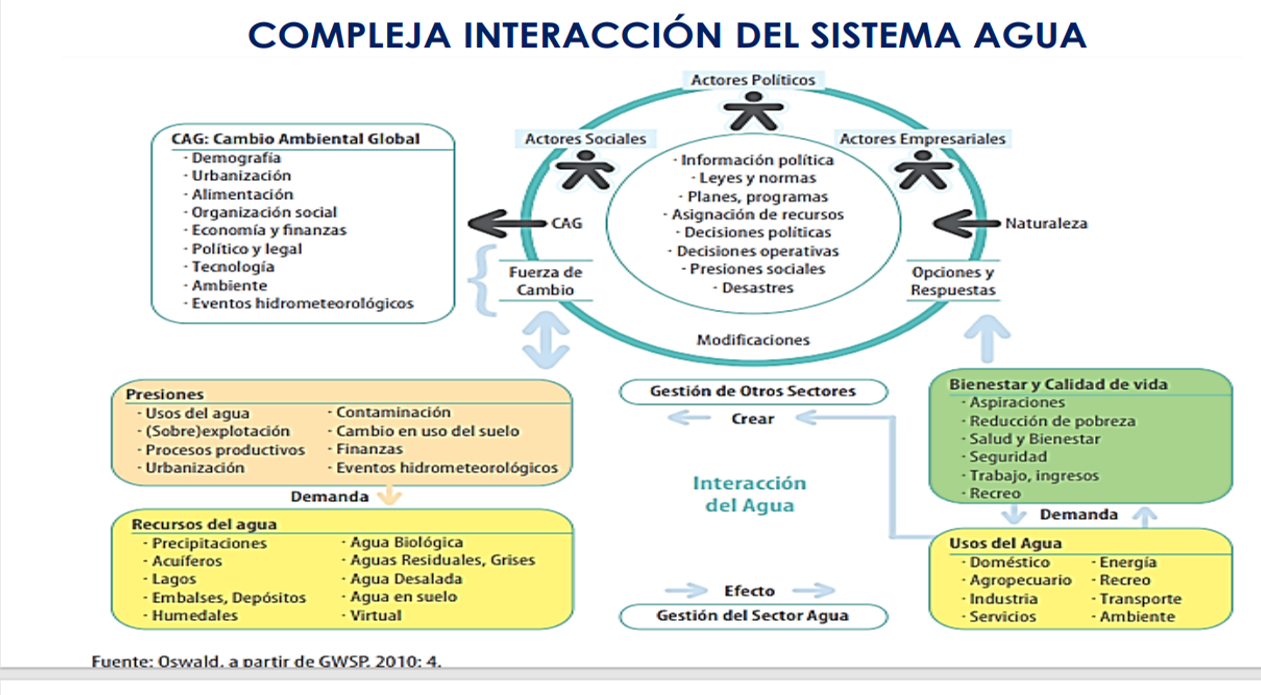
\includegraphics[width=0.5\textwidth]{ar11.png}
  \caption{Compleja interacción del sistema agua\cite{bogardi2016water}}
  \label{ar11}
\end{figure}
\subsubsection{Mejora de la gestión del agua en la explotación agrícola}
Cuando hay poca disponibilidad de agua es obligatorio mejorar la gestión o ausencia de irrigación. También se recomienda integrar prácticas para la conservación del agua e incentivos económicos para influir en el volumen total del consúmo y en las pautas de uso del agua. Elevar al máximo la producción agrícola por unidad de tierra contribuye a optimizar el rendimiento por unidad de volumen del agua.

Es necesario aumentar la eficiencia energética de las plantas de desalinización, ésta ha sido una solución de alto consumo energético a la escasez de agua; es viable en regiones con disponibilidad de recursos y se precisa el fomento de tecnologías en energías renovables.

La escasez complica la seguridad alimentaria y la contaminación, por lo que los gobiernos tienen que tomar medidas que consideren los efectos a medio y largo plazo, debe aplicarse una gestión integral con un enfoque práctico y de sentido común para la supervisión de los recursos naturales, teniendo en cuenta consideraciones económicas, culturales y los objetivos ecológicos

Las deficiencias en la distribución tienen un impacto serio en la utilización de los recursos, la salud y la economía.

Con relación a la escasez, plantear soluciones a nivel de cuenca mediante programas de gestión integrada del agua; fortalecer a todas las organizaciones que
participan en la toma de decisiones, y simplificar los instrumentos económicos, sociales y políticos que las soporten.

En materia de agua subterránea, fomentar la recarga de los acuíferos mediante
la recarga virtual, la reinyección física y la aplicación de la Ley para evitar pozos
clandestinos, y buscar nuevas fuentes para sustituir el agua que se extrae de un
acuífero de zonas donde no se causen impactos ambientales de consideración.

Asimismo, mejorar la eficiencia de los Distritos de Riego, Unidades de Riego y
Organismos Operadores de Agua Potable y Saneamiento.

Con relación al cambio climático, es necesario que el país invierta más en investigación y desarrollo; que se establezcan mecanismos reales de compromiso por parte de los involucrados con este fenómeno, y que se utilicen datos y modelos mexicanos en los procesos de planteamiento de escenarios.

Se propone impulsar de inversión en investigación científica; promover el posgrado en todo el país; incrementar los recursos asignados al Conacyt; impulsar la descentralización de actividades científicas y tecnológicas.

Finalmente, se hace una propuesta para incrementar la oferta de agua mediante el reúso, el agua virtual, la desalación y el aprovechamiento de la humedad del suelo.

Algunas propuestas para solucionar los problemas de contaminación son aumentar la eficiencia de los organismos operadores; fortalecer su autosuficiencia financiera; el tratamiento de sus aguas residuales y su reúso en forma sustentable técnica y económicamente; orientar el crecimiento de las ciudades hacia zonas con disponibilidad de agua, y lograr que el tratamiento de las aguas residuales esté en la agenda de las instancias federal, estatal y municipal.

A nivel de cuenca, es necesario realizar evaluaciones de la contaminación difusa aportada por ciudades y zonas agrícolas. Y en materia de contaminación puntual, se debe tratar y reusar al menos 60 % de las aguas residuales recolectadas, así como mejorar la eficiencia de las plantas construidas. 

Para mejorar la administración del agua, se debe hacer una nueva Ley de Aguas
Nacionales e incrementar los recursos presupuestales y financieros para el sector
agua; fortalecer la capacidad institucional de la Comisión Nacional del Agua;
impulsar el proceso de descentralización; reforzar a las asociaciones de usuarios
del agua, e incrementar la participación del sector en el concierto internacional.

Es necesario el ordenamiento ecológico de las cuencas y el alineamiento de
competencias de las instancias federales, estatales y municipales responsables de
ello en el país, pues son muchas dependencias las que están involucradas en la
solución de un problema tan complejo.

Urge iniciar tareas de reforestación en las partes altas de las cuencas; establecer zonas de riesgo (atlas de riesgo) de áreas inundables, zonas federales, cauces nacionales, humedales y barrancas, y desarrollar una arquitectura de regiones inundables.

\subsubsection{Conductividad eléctrica}
Es una expresión numérica de la capacidad de una solución para transportar una corriente eléctrica. Esta capacidad de la precencia de iones, de us concentración total, de su movilidad, valencia y concentraciones relaticas, así como de la temperatura.

La determinación de conductividad es de gran importancia pues da una idea del grado de mineralización del agua natural, potable, residual, residual tratada, de proceso o bien del agua para se usada en el laboratorio en análisis de rutina o para trabajos de investigación. El valor de conductividad es un parámetro regulado por límites máximos permisibles en descargas de aguas residuales al alcantarillado o a cuerpos receptores, también es un parámetro de calidad del agua para usos y actividades agrícolas, para contacto primario y para el consumo humano.
\subsubsection{Potencial de Hidrógeno}
El pH es una medida que indica la acidez del agua, el rango varía de 0 a14, siendo 7 el promedio neutral. El pH se puede ver afectado por la sedimentación atmosférica (lluvia ácida) provenientes de industrias y transporte, los vertidos de aguas residuales, los drenajes de las minas y el tipo de rocas que forman el lecho de la masa de agua estudiada.




































